\begin{frame}{$\EoL[k]$}
    \begin{minipage}{0.5 \linewidth}
        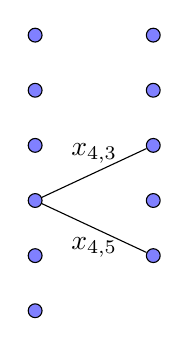
\begin{tikzpicture}[>=latex]

    \foreach \i in {1, 2, ..., 6}{
        \node[draw, circle, fill = blue!50, inner sep = 0pt, minimum size = 5pt]
            (a\i) at (0, -0.7 * \i) {};
    }

    \foreach \i in {1, 2, ..., 5}{
        \node[draw, circle, fill = blue!50, inner sep = 0pt, minimum size = 5pt]
            (b\i) at (1.5, -0.7 * \i) {};
    }
    
    \draw (a4) -- (b3) node[midway, above] {$x_{4, 3}$};
    \draw (a4) -- (b5) node[midway, below] {$x_{4, 5}$};
\end{tikzpicture}
    \end{minipage}%
    \begin{minipage}{0.5 \linewidth}
        \pause
        \pause
        \begin{itemize}
            \item $v: ~ \sum\limits_{e \in E^{in}_v} x_{e} - \sum\limits_{e \in E^{out}_v} x_{e} = c(v)$
                \textcolor{red}{$(\mathbb{R})$};
            \item $\sum\limits_{v} c(v) = k$ \textcolor{red}{$(\mathbb{R})$};
            \item $k \neq 0 \Rightarrow \EoL[k]$ is unsat. 
        \end{itemize}
    \end{minipage}

    \pause
    \begin{lemma}
        $\EoL[1]$ has a low degree $\NS$-proof over any field.
    \end{lemma}
\end{frame}

\begin{frame}{Mystery of lines}

    \begin{lemma}[1]
        \begin{itemize}
            \item $\EoL[1]$ has a low degree $\NS$-proof over any field;
            \item $\forall k, \EoL[k]$ has a low degree $\NS$-proof over $\mathbb{R}$.
        \end{itemize}
    \end{lemma}

    \pause

    \begin{lemma}[2]
        $G$ is $(n, d, \alpha)$-expander $\Rightarrow$ $w(\EoL[1]) = \Omega(n)$.
    \end{lemma}

    \pause

    \begin{lemma}[3]
        $k = \mathrm{char}(\mathbb{F})^{\ell} \Rightarrow \exists G$, there is no $2^{\ell} =
        \Omega(\sqrt{n})$ degree $\NS$-proof of $\EoL[k]$ over $\mathbb{F}$.
    \end{lemma}

    \begin{itemize}
        \item $(1), (2) \Rightarrow$ separation between $mSP$ and monotone circuits;
        \item $(1), (3) \Rightarrow$ $mSP$ over $\mathbb{R}$ can be stronger than $mSP$ over fields with
            $\mathrm{char} > 0$. 
    \end{itemize}

\end{frame}


\begin{frame}{Open problems}

    \begin{enumerate}
        \item $k = \mathrm{char}(\mathbb{F})^{\ell}$. Can we prove $\Omega(n)$-degree lower bound?
        \item $k = \mathrm{char}(\mathbb{F})^{\ell}$. Polynomial calculus lower bounds?
        \item Model that can capture $mSP$ and monotone circuits simultaneously?
    \end{enumerate}
\end{frame}